\documentclass{standalone}
\usepackage{tikz}
\usetikzlibrary{patterns, positioning}
\usepackage[sfdefault]{ClearSans} %% option 'sfdefault' activates Clear Sans as the default text font
\usepackage[T1]{fontenc}

\begin{document}
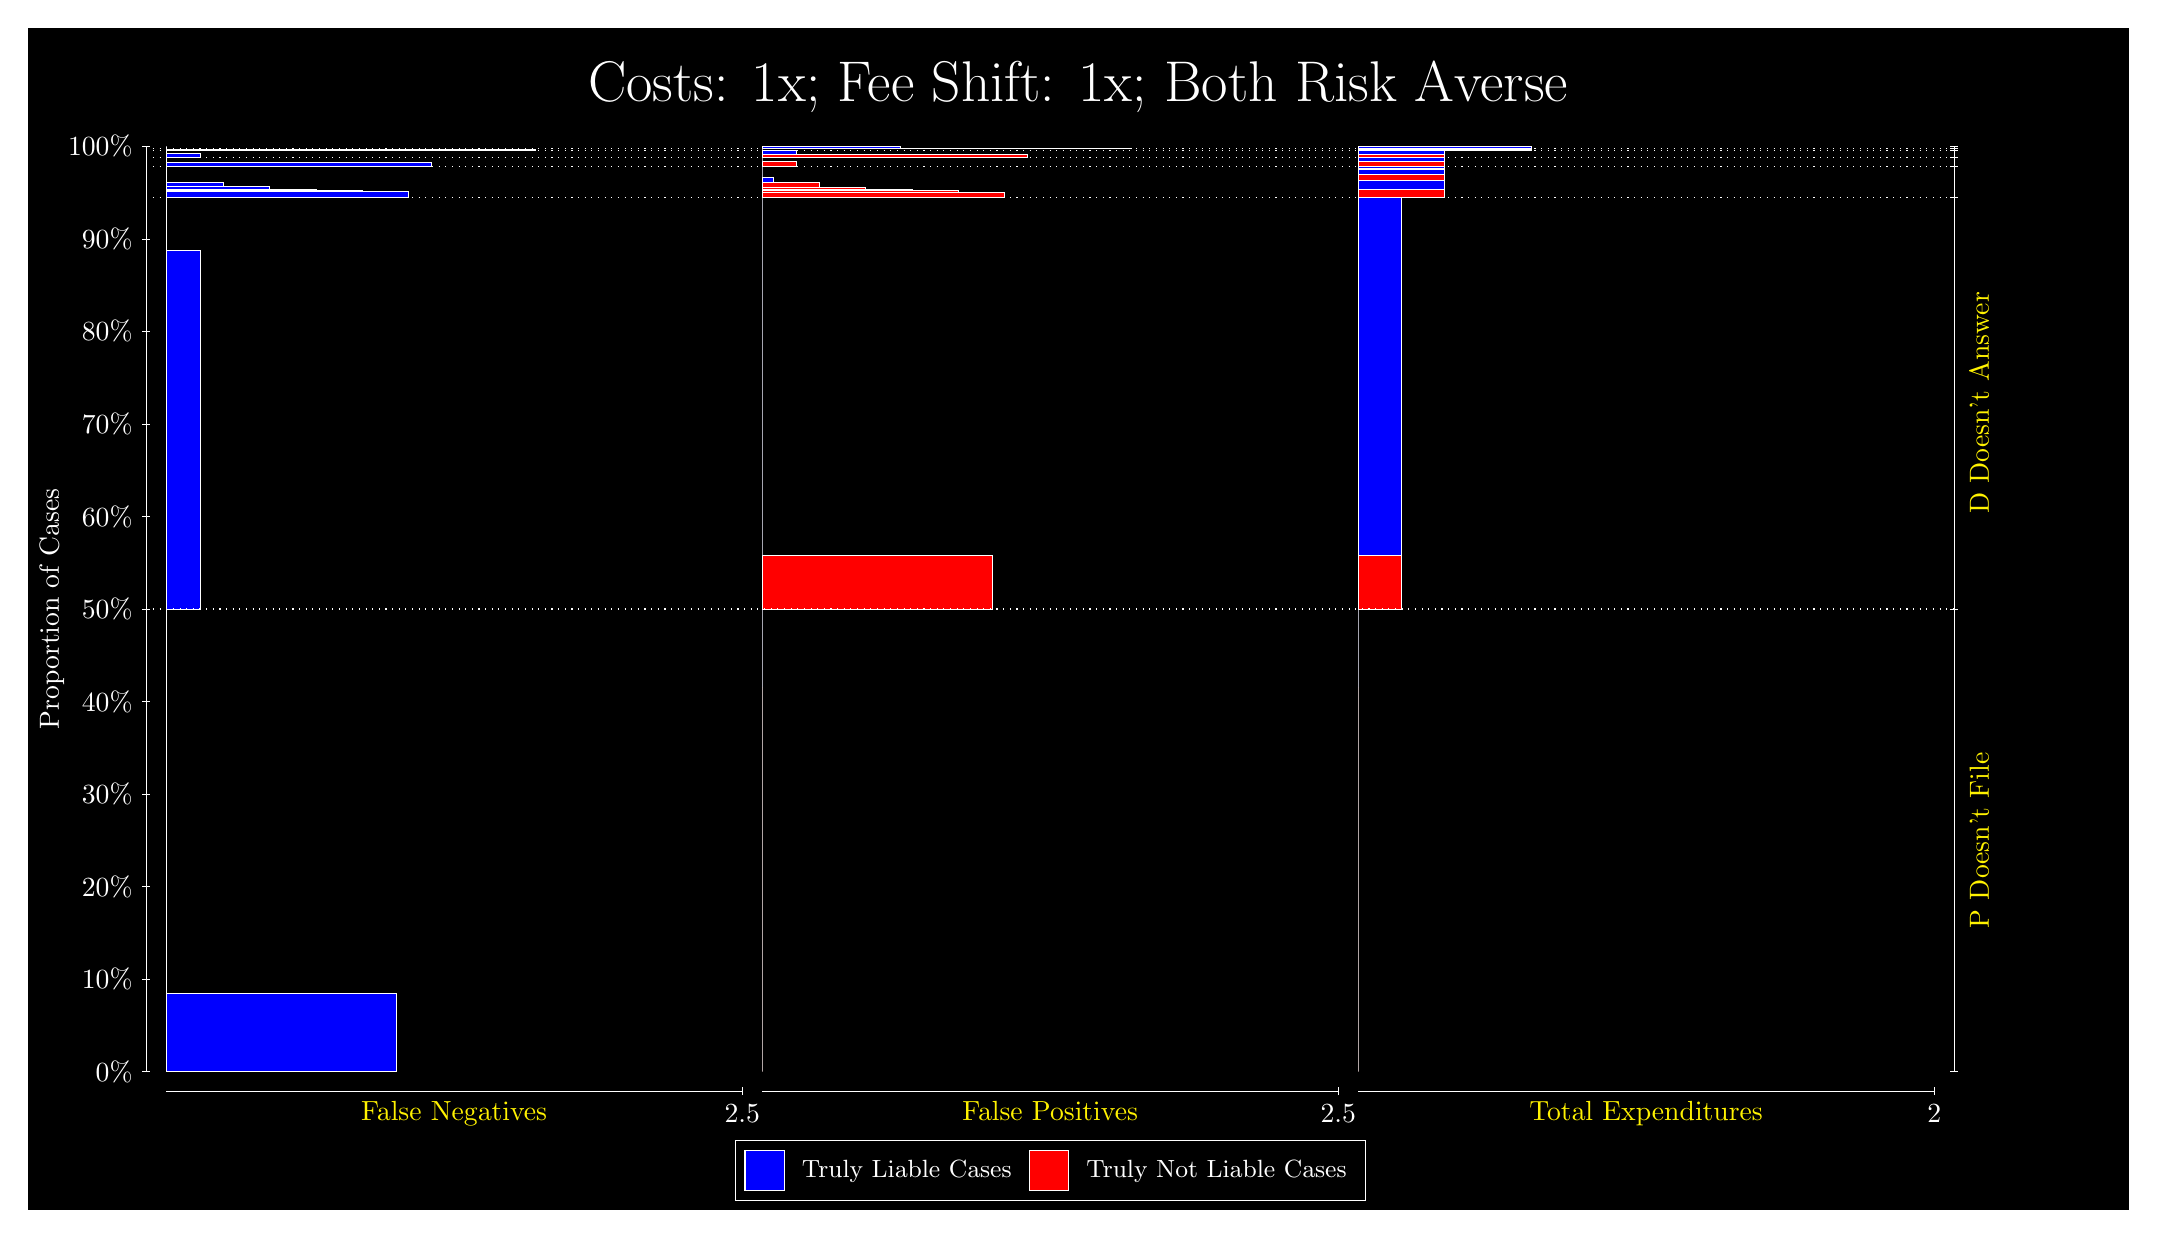
\begin{tikzpicture}
\draw[fill=black] (0,0) rectangle (26.667,15);
\draw[text=white] (0,13.5) rectangle (26.667,15) node[midway] {\huge Costs: 1x; Fee Shift: 1x; Both Risk Averse};
\draw[white, very thin] (1.5,1.75) -- (1.5,13.5);
\node[rotate=90, text=white, anchor=center] at (0.3, 7.625) {Proportion of Cases};
\draw[white, very thin] (1.45,1.75) -- (1.55,1.75);
\node[text=white, anchor=east] at (1.45, 1.75) {0\%};
\draw[white, very thin] (1.45,2.925) -- (1.55,2.925);
\node[text=white, anchor=east] at (1.45, 2.925) {10\%};
\draw[white, very thin] (1.45,4.1) -- (1.55,4.1);
\node[text=white, anchor=east] at (1.45, 4.1) {20\%};
\draw[white, very thin] (1.45,5.275) -- (1.55,5.275);
\node[text=white, anchor=east] at (1.45, 5.275) {30\%};
\draw[white, very thin] (1.45,6.45) -- (1.55,6.45);
\node[text=white, anchor=east] at (1.45, 6.45) {40\%};
\draw[white, very thin] (1.45,7.625) -- (1.55,7.625);
\node[text=white, anchor=east] at (1.45, 7.625) {50\%};
\draw[white, very thin] (1.45,8.8) -- (1.55,8.8);
\node[text=white, anchor=east] at (1.45, 8.8) {60\%};
\draw[white, very thin] (1.45,9.975) -- (1.55,9.975);
\node[text=white, anchor=east] at (1.45, 9.975) {70\%};
\draw[white, very thin] (1.45,11.15) -- (1.55,11.15);
\node[text=white, anchor=east] at (1.45, 11.15) {80\%};
\draw[white, very thin] (1.45,12.325) -- (1.55,12.325);
\node[text=white, anchor=east] at (1.45, 12.325) {90\%};
\draw[white, very thin] (1.45,13.5) -- (1.55,13.5);
\node[text=white, anchor=east] at (1.45, 13.5) {100\%};

\draw[white, very thin] (24.457,1.75) -- (24.457,13.5);
\draw[white, very thin] (24.407,1.75) -- (24.507,1.75);
\node[anchor=west] at (24.407, 1.75) {};
\draw[white, very thin] (24.407,7.6244) -- (24.507,7.6244);
\node[anchor=west] at (24.407, 7.6244) {};
\draw[white, very thin] (24.407,12.855) -- (24.507,12.855);
\node[anchor=west] at (24.407, 12.855) {};
\draw[white, very thin] (24.407,13.242) -- (24.507,13.242);
\node[anchor=west] at (24.407, 13.242) {};
\draw[white, very thin] (24.407,13.359) -- (24.507,13.359);
\node[anchor=west] at (24.407, 13.359) {};
\draw[white, very thin] (24.407,13.45) -- (24.507,13.45);
\node[anchor=west] at (24.407, 13.45) {};
\draw[white, very thin] (24.407,13.47) -- (24.507,13.47);
\node[anchor=west] at (24.407, 13.47) {};
\draw[white, very thin] (24.407,13.5) -- (24.507,13.5);
\node[anchor=west] at (24.407, 13.5) {};

\draw[white, very thin, fill=blue] (1.75,1.75) rectangle (4.6775,2.7431);
\draw[white, very thin, fill=red] (1.75,2.7431) rectangle (1.75,7.6244);
\draw[white, very thin, fill=blue] (1.75,7.6244) rectangle (2.1891,12.179);
\draw[white, very thin, fill=red] (1.75,12.179) rectangle (1.75,12.855);
\draw[white, very thin, fill=blue] (1.75,12.855) rectangle (4.8239,12.927);
\draw[white, very thin, fill=blue] (1.75,12.927) rectangle (4.2384,12.942);
\draw[white, very thin, fill=blue] (1.75,12.942) rectangle (3.9457,12.942);
\draw[white, very thin, fill=blue] (1.75,12.942) rectangle (3.6529,12.958);
\draw[white, very thin, fill=blue] (1.75,12.958) rectangle (3.0674,12.987);
\draw[white, very thin, fill=blue] (1.75,12.987) rectangle (2.4819,13.048);
\draw[white, very thin, fill=red] (1.75,13.048) rectangle (1.75,13.242);
\draw[white, very thin, fill=blue] (1.75,13.242) rectangle (5.1167,13.297);
\draw[white, very thin, fill=red] (1.75,13.297) rectangle (1.75,13.359);
\draw[white, very thin, fill=blue] (1.75,13.359) rectangle (2.1891,13.411);
\draw[white, very thin, fill=red] (1.75,13.411) rectangle (1.75,13.45);
\draw[white, very thin, fill=blue] (1.75,13.45) rectangle (6.4341,13.458);
\draw[white, very thin, fill=red] (1.75,13.458) rectangle (1.75,13.47);
\draw[white, very thin, fill=red] (1.75,13.47) rectangle (1.75,13.479);
\draw[white, very thin, fill=blue] (1.75,13.479) rectangle (1.75,13.5);
\draw[white, very thin, fill=red] (9.3189,1.75) rectangle (9.3189,6.6314);
\draw[white, very thin, fill=blue] (9.3189,6.6314) rectangle (9.3189,7.6244);
\draw[white, very thin, fill=red] (9.3189,7.6244) rectangle (12.246,8.3004);
\draw[white, very thin, fill=blue] (9.3189,8.3004) rectangle (9.3189,12.855);
\draw[white, very thin, fill=red] (9.3189,12.855) rectangle (12.393,12.913);
\draw[white, very thin, fill=red] (9.3189,12.913) rectangle (11.807,12.942);
\draw[white, very thin, fill=red] (9.3189,12.942) rectangle (11.222,12.958);
\draw[white, very thin, fill=red] (9.3189,12.958) rectangle (10.929,12.959);
\draw[white, very thin, fill=red] (9.3189,12.959) rectangle (10.636,12.974);
\draw[white, very thin, fill=red] (9.3189,12.974) rectangle (10.051,13.049);
\draw[white, very thin, fill=blue] (9.3189,13.049) rectangle (9.4652,13.11);
\draw[white, very thin, fill=blue] (9.3189,13.11) rectangle (9.3189,13.242);
\draw[white, very thin, fill=red] (9.3189,13.242) rectangle (9.758,13.305);
\draw[white, very thin, fill=blue] (9.3189,13.305) rectangle (9.3189,13.359);
\draw[white, very thin, fill=red] (9.3189,13.359) rectangle (12.686,13.399);
\draw[white, very thin, fill=blue] (9.3189,13.399) rectangle (9.758,13.45);
\draw[white, very thin, fill=red] (9.3189,13.45) rectangle (9.3189,13.463);
\draw[white, very thin, fill=blue] (9.3189,13.463) rectangle (9.3189,13.47);
\draw[white, very thin, fill=red] (9.3189,13.47) rectangle (14.003,13.479);
\draw[white, very thin, fill=blue] (9.3189,13.479) rectangle (11.075,13.5);
\draw[white, very thin, fill=red] (16.888,1.75) rectangle (16.888,6.6314);
\draw[white, very thin, fill=blue] (16.888,6.6314) rectangle (16.888,7.6244);
\draw[white, very thin, fill=red] (16.888,7.6244) rectangle (17.437,8.3004);
\draw[white, very thin, fill=blue] (16.888,8.3004) rectangle (17.437,12.855);
\draw[white, very thin, fill=red] (16.888,12.855) rectangle (17.986,12.958);
\draw[white, very thin, fill=blue] (16.888,12.958) rectangle (17.986,13.064);
\draw[white, very thin, fill=red] (16.888,13.064) rectangle (17.986,13.139);
\draw[white, very thin, fill=blue] (16.888,13.139) rectangle (17.986,13.211);
\draw[white, very thin, fill=red] (16.888,13.211) rectangle (17.986,13.226);
\draw[white, very thin, fill=blue] (16.888,13.226) rectangle (17.986,13.242);
\draw[white, very thin, fill=red] (16.888,13.242) rectangle (17.986,13.305);
\draw[white, very thin, fill=blue] (16.888,13.305) rectangle (17.986,13.359);
\draw[white, very thin, fill=red] (16.888,13.359) rectangle (17.986,13.399);
\draw[white, very thin, fill=blue] (16.888,13.399) rectangle (17.986,13.45);
\draw[white, very thin, fill=red] (16.888,13.45) rectangle (19.083,13.463);
\draw[white, very thin, fill=blue] (16.888,13.463) rectangle (19.083,13.47);
\draw[white, very thin, fill=red] (16.888,13.47) rectangle (19.083,13.479);
\draw[white, very thin, fill=blue] (16.888,13.479) rectangle (19.083,13.5);
\draw[white, dotted] (1.5,7.6244) -- (24.457,7.6244);
\draw[white, dotted] (1.5,12.855) -- (24.457,12.855);
\draw[white, dotted] (1.5,13.242) -- (24.457,13.242);
\draw[white, dotted] (1.5,13.359) -- (24.457,13.359);
\draw[white, dotted] (1.5,13.45) -- (24.457,13.45);
\draw[white, dotted] (1.5,13.47) -- (24.457,13.47);
\draw[white, very thin] (1.75,1.5) -- (9.0689,1.5);
\node[text=yellow, anchor=north] at (5.4094, 1.5) {False Negatives};
\draw[white, very thin] (9.0689,1.45) -- (9.0689,1.55);
\node[text=white, anchor=north] at (9.0689, 1.45) {2.5};

\draw[white, very thin] (9.3189,1.5) -- (16.638,1.5);
\node[text=yellow, anchor=north] at (12.978, 1.5) {False Positives};
\draw[white, very thin] (16.638,1.45) -- (16.638,1.55);
\node[text=white, anchor=north] at (16.638, 1.45) {2.5};

\draw[white, very thin] (16.888,1.5) -- (24.207,1.5);
\node[text=yellow, anchor=north] at (20.547, 1.5) {Total Expenditures};
\draw[white, very thin] (24.207,1.45) -- (24.207,1.55);
\node[text=white, anchor=north] at (24.207, 1.45) {2};

\node[text=yellow, centered, rotate=90] at (24.777, 4.6872) {P Doesn't File};
\node[text=yellow, centered, rotate=90] at (24.777, 10.24) {D Doesn't Answer};






\draw (12.978300999999998,1.5) node[draw=none] (baseCoordinate) {};
\begin{scope}[align=center]
        \matrix[scale=0.5, draw=white, below=0.5cm of baseCoordinate, nodes={draw}, column sep=0.1cm]{
            \node[rectangle, draw, minimum width=0.5cm, minimum height=0.5cm, fill=blue] {}; &
            \node[draw=none, font=\small, text=white] (B) {Truly Liable Cases}; &
            \node[rectangle, draw, minimum width=0.5cm, minimum height=0.5cm, fill=red] {}; &
            \node[draw=none, font=\small, text=white] (B) {Truly Not Liable Cases}; \\
            };
\end{scope}

\end{tikzpicture}
\end{document}